\documentclass{beamer}

\author[D. Abercrombie]{
  Daniel Abercrombie
}

\title{\bf \sffamily Consistency Check Design and Use}
\date{October 13, 2017}

\usecolortheme{dove}

\usefonttheme{serif}
\setbeamerfont{frametitle}{series=\bf\sffamily}
\setbeamertemplate{frametitle}[default][center]
\usepackage{tabularx}
\usepackage[normalem]{ulem}

\setbeamertemplate{navigation symbols}{}
\usepackage{graphicx}
\usepackage{color}
\setbeamertemplate{footline}[text line]{\parbox{1.083\linewidth}{\footnotesize \hfill \insertshortauthor \hfill \insertpagenumber /\inserttotalframenumber}}
\setbeamertemplate{headline}[text line]{\footnotesize \textcolor{blue}{\bf \sffamily \hfill \insertsection}}

\IfFileExists{/Users/dabercro/GradSchool/Presentations/MIT-logo.pdf}
             {\logo{\includegraphics[height=0.5cm]{/Users/dabercro/GradSchool/Presentations/MIT-logo.pdf}}}
             {\logo{\includegraphics[height=0.5cm]{/home/dabercro/MIT-logo.pdf}}}

\usepackage{changepage}

\newcommand{\link}[2]{\href{#2}{\textcolor{blue}{\underline{#1}}}}
\newcommand{\clink}[2]{\link{#1}{http://t3serv001.mit.edu/~dabercro/redir/?k=#2}}}
\newcommand{\self}{\textcolor{blue}{self} }

\newcommand{\twofigs}[4]{
  \begin{columns}
    \begin{column}{0.5\linewidth}
      \centering
      \textcolor{blue}{#1} \\
      \includegraphics[width=\linewidth]{#2}
    \end{column}
    \begin{column}{0.5\linewidth}
      \centering
      \textcolor{blue}{#3} \\
      \includegraphics[width=\linewidth]{#4}
    \end{column}
  \end{columns}
}

\newcommand{\fourfigs}[8]{
  \begin{columns}
    \begin{column}{0.15\linewidth}
    \end{column}
    \begin{column}{0.35\linewidth}
      \centering
      \textcolor{blue}{#1} \\
      \includegraphics[width=0.8\linewidth]{#2} \\
      \textcolor{blue}{#3} \\
      \includegraphics[width=0.8\linewidth]{#4}
    \end{column}
    \begin{column}{0.35\linewidth}
      \centering
      \textcolor{blue}{#5} \\
      \includegraphics[width=0.8\linewidth]{#6} \\
      \textcolor{blue}{#7} \\
      \includegraphics[width=0.8\linewidth]{#8}
    \end{column}
    \begin{column}{0.15\linewidth}
    \end{column}
  \end{columns}
}

\usepackage{listings}

\lstset{
  basicstyle=\scriptsize\ttfamily
}

\usepackage{tikz}
\usetikzlibrary{arrows, positioning, intersections}

\tikzset{
  goodstep/.style={
    minimum width=2cm, 
    minimum height=1cm, 
    align=center, 
    draw=black,
    rounded corners=0.1cm,
    font=\scriptsize
  },
  async/.style={
    minimum width=2cm, 
    minimum height=1cm, 
    align=center, 
    draw=blue,
    rounded corners=0.1cm,
    font=\scriptsize
  },
  direct/.style={
    minimum width=2.5cm, 
    minimum height=0.75cm, 
    align=center,
    draw=black,
    rounded corners=0.25cm
  },
  note/.style={
    minimum width=2cm, 
    minimum height=1cm, 
    align=center
  },
  arrow/.style={draw,thick,->,>=stealth}
}

\graphicspath{{../171002/figs/}{figs/}}

\begin{document}

\begin{frame}
  \titlepage
\end{frame}

\begin{frame}
  \frametitle{Outline}
  \tableofcontents
\end{frame}

\section{Motivation}

\begin{frame}
  \frametitle{Outline}
  \textcolor{red}{Motivation for the outline slides is from watching J-Lab talks.}
  \tableofcontents[currentsection]
\end{frame}

\begin{frame}
  \frametitle{We want to know what files are actually at each site}

  We compare what is physically at a site with what is
  expected to be there according to an inventory database.

  \begin{itemize}
  \item Sites may be missing files
    \begin{itemize}
    \item Can cause transfers to fail if source is invalid
    \item Sites are chosen incorrectly for production jobs
      that assume a local file
    \item Last disk copy might actually not be present,
      causing a delay when requested by a user
    \end{itemize}
  \item Some files may not be accounted for in our inventory
    \begin{itemize}
    \item Will not be used (besides accidentially through AAA)
    \item Wasting disk space
    \end{itemize}
  \end{itemize}

\end{frame}

\begin{frame}
  \frametitle{There is room for improving the old method}

  \begin{itemize}
  \item When?
    \begin{itemize}
    \item T0/T1 sites are checked twice a year
    \item T2 checked when problem suspected, on request
    \end{itemize}
  \item How?
    \begin{itemize}
    \item Contact site admins
    \item Wait
    \item Download site content
    \item Compare physical content with inventory
      \begin{itemize}
      \item Via some method that may be better than mine
      \end{itemize}
    \item Give admins lists of orphans and locally invalidate missing
    \item Wait
    \item Fixed!
    \end{itemize}
  \end{itemize}

  Both of these processes are time-intensive, and manual \\
  (\emph{i.e.} requires emails, waiting, and other keystrokes). \\
  We should be able to delegate these tasks to a machine.

\end{frame}

\section{Comparison Algorithm Design}

\begin{frame}
  \frametitle{Outline}
  \tableofcontents[currentsection]
\end{frame}

\begin{frame}
  \frametitle{What's the best way to compare lists of files?}

  Answer: Ordered lists
  \begin{itemize}
  \item but those are boring
  \item and not flexible
  \item technically not optimal when skipping groups of new files
  \end{itemize}

  Goals:
  \begin{itemize}
  \item List inventory fast
  \item List sites with parallel (to be fast) processes
  \item Do comparison (fast)
  \item Get overview of disk utilization (whenever it's ready)
    \begin{itemize}
    \item Directory counting would be hard with linear lists
    \end{itemize}
  \end{itemize}

\end{frame}

\begin{frame}
  \frametitle{Modified answer: trees}

  \begin{center}
    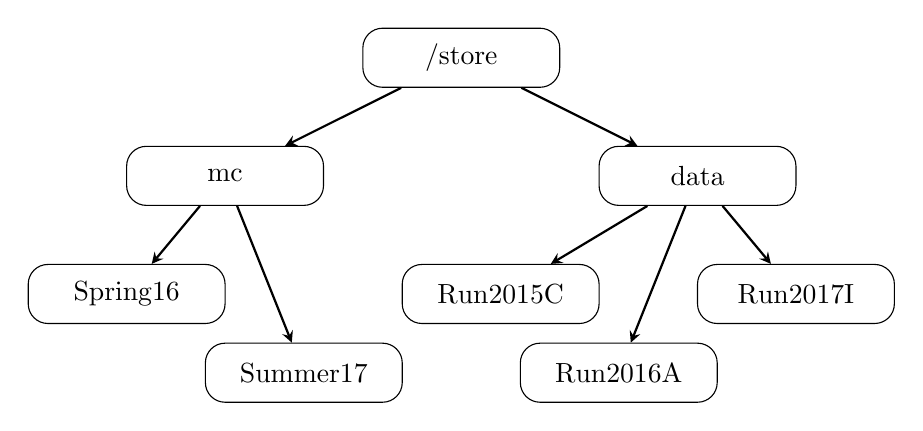
\begin{tikzpicture}[every edge/.style={arrow}]
      \node (root) [direct] at (0,10) {/store};
      \node (a) at (-3, 8.5) [direct] {mc};
      \node (aa) at (-4.25, 7) [direct] {Spring16};
      \node (ab) at (-2, 6) [direct] {Summer17};
      \node (b) at (3, 8.5) [direct] {data};
      \node (ba) at (0.5, 7) [direct] {Run2015C};
      \node (bb) at (2, 6) [direct] {Run2016A};
      \node (bc) at (4.25, 7) [direct] {Run2017I};
      \path
      (root) edge (a)
      (root) edge (b)
      (a) edge (aa)
      (a) edge (ab)
      (b) edge (ba)
      (b) edge (bb)
      (b) edge (bc)
      ;
  \end{tikzpicture}
  \end{center}

  \vfill
  \begin{itemize}
  \item After listing ``/store'', an arbitrary number of workers can go around listing each unlisted node until the queue is done
  \item A lot of recursive algorithms become useful by induction
  \end{itemize}

\end{frame}

\begin{frame}
  \frametitle{Data members of a directory}

  Directory information consists of the following:
  \begin{itemize}
  \item name (not absolute path, just the name of this directory)
  \item timestamp of when Python object created
  \item modtime of directory
  \item list of subdirectories
  \item list of files, which are dictionaries with:
    \begin{itemize}
    \item name
    \item size
    \item modtime
    \item hash of name and size
    \item flag of whether this can be listed as extra
    \end{itemize}
  \item hash of name, comparable subdirectory hashes, \\
    and comparable file hashes
  \item flag of whether this can be listed as extra
  \end{itemize}

\end{frame}

\begin{frame}
  \frametitle{What can be extra?}

  \begin{itemize}
  \item Files are listed as extra when too much older than directories timestamp \\
    (creation time of Python object)
  \item Directories can be compared when:
    \begin{itemize}
    \item At least one file is deletable
    \item OR at least one subdirectory can be compared
    \item OR is empty and is much older than creation
    \end{itemize}
  \end{itemize}

\end{frame}

\begin{frame}
  \frametitle{For my next trick, I copy Donald Knuth}

  Recursive comparison algorithm
  \vfill

  \begin{center}
  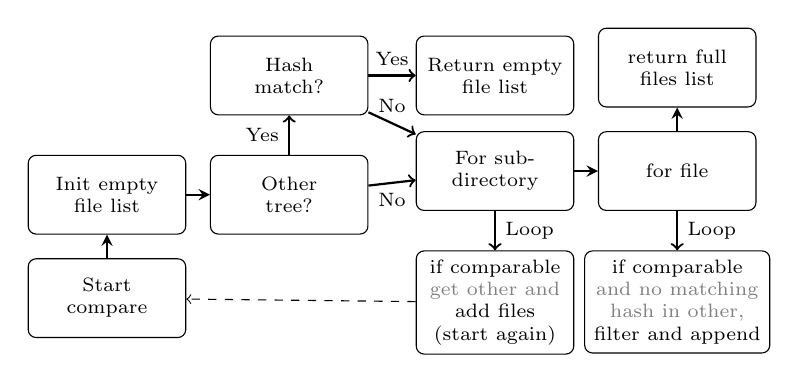
\begin{tikzpicture}[node distance=0.3cm, every edge/.style={arrow}]
    \node (start) [goodstep] at (0,0) {Init empty \\ file list};
    \node (realstart) [goodstep, below=of start] {Start \\ compare};
    \node (treecheck) [goodstep, right=of start] {Other \\ tree?};
    \node (tree) [goodstep, above=0.5cm of treecheck] {Hash \\ match?};
    \draw [->, thick] (treecheck) -- node [font=\scriptsize, left] {Yes} (tree);
    \node (nohash) [goodstep, below right=0.2cm and 0.6cm of tree] {For sub- \\ directory};
    \draw [->, thick] (tree) -- node [font=\scriptsize, above] {No} (nohash);
    \node (subdir) [goodstep, below=0.5cm of nohash] {if comparable \\
      \textcolor{gray}{get other and} \\
      add files \\ (start again)};
    \node (files) [goodstep, right=of nohash] {for file};
    \node (checkfile) [goodstep, below=0.5cm of files] {if comparable \\
      \textcolor{gray}{and no matching} \\
      \textcolor{gray}{hash in other,} \\ filter and append};
    \draw [->, thick] (treecheck) -- node [font=\scriptsize, below] {No} (nohash);
    \draw [->, dashed] (subdir) -- (realstart);
    \draw [->, thick] (nohash) -- node [font=\scriptsize, right] {Loop} (subdir);
    \draw [->, thick] (files) -- node [font=\scriptsize, right] {Loop} (checkfile);
    \node (final) [goodstep, above=of files] {return full \\ files list};
    \node (match) [goodstep, right=0.6cm of tree] {Return empty \\ file list};
    \draw [->, thick] (tree) -- node [font=\scriptsize, above] {Yes} (match);
    \path
    (realstart) edge (start)
    (start) edge (treecheck)
    (nohash) edge (files)
    (files) edge (final)
    ;
  \end{tikzpicture}
  \end{center}

  \vfill
  The MMIX for this algorithm is left as an exercise.
\end{frame}

\section{Development Philosophy}

\begin{frame}
  \frametitle{Outline}
  \tableofcontents[currentsection]
\end{frame}

\begin{frame}
  \frametitle{The internet is full of advice}
  I was going to say
  ``cocky developers who (rightly) think that they know better than kids these days''
  instead of ``advice'', but that wouldn't have fit in the slide title.

  \vfill

  Code is only as good as its:
  \begin{itemize}
  \item Documentation
  \item Comments
  \item Tests
  \item License?
  \item Man hours over age
  \end{itemize}

\end{frame}

\begin{frame}
  \frametitle{Make tool comfy and easy to wear}

  \begin{itemize}
  \item Should work in every possible environment
    \begin{itemize}
    \item Good for testing or giving to Brian
    \item Environment variables are powerful
    \item For everything else, there's \sout{Mast} a configuration file
    \end{itemize}
  \item Function signatures should be simple: \\
    \lstinputlisting{cmd.txt}
    \begin{enumerate}
    \item Decide on signature
    \item Do not write function
    \item Write tests to prove function will behave properly
    \item Write function until passes tests
    \end{enumerate}
  \item If you really need to be more specific,
    tests will keep your default behavior the same
  \item No one will complain that you broke their code by updating yours
  \end{itemize}

\end{frame}

\begin{frame}
  \frametitle{How to kill bugs so they stay dead}

  Sometimes (basically always while working alone or on a small team),
  a case will come up that you did not think to test for.

  I have adopted the following procedure.

  \begin{enumerate}
  \item Notice bug
  \item Parse logs or add debuging output
    (no other code changes)
    to diagnose problem
  \item Write test that fails because of problem
  \item Once test fails, fix code to make test pass
  \item Append new test to all tests
  \item Now run all tests again
  \item Pull request and merge
  \item Run all tests
  \item Production
  \end{enumerate}

\end{frame}

\section{Real World Implementation}

\begin{frame}
  \frametitle{Outline}
  \textcolor{red}{Unfortunately, this is stuff that I have to test by hand.}
  \tableofcontents[currentsection]
\end{frame}

\begin{frame}
  \frametitle{Get site content through XRootD}

  \begin{center}
  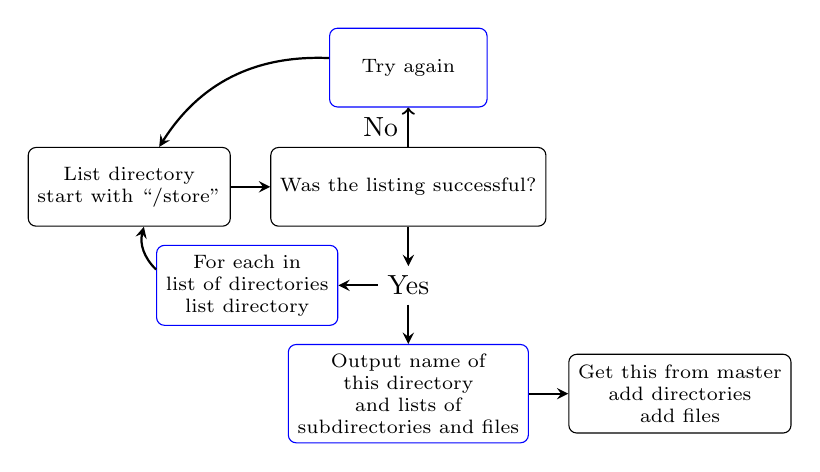
\begin{tikzpicture}[node distance=0.5cm, every edge/.style={arrow}]
  \node (start) [goodstep] at (0, 0) {List directory \\ start with ``/store''};
  \node (good) [goodstep, right=of start] {Was the listing successful?};
  \node (yes) [below=of good] {Yes};
  \node (outqueue) [async, below=of yes] {Output name of \\ this directory \\
    and lists of \\ subdirectories and files};
  \node (inqueue) [async, left=of yes] {For each in \\ list of directories \\
    list directory};
  \node (master) [goodstep, right=of outqueue] {Get this from master \\
    add directories \\ add files};
  \node (try) [async, above=of good] {Try again};
  \draw [->, thick] (good) -- node [left] {No} (try);
  \path
  (start) edge (good)
  (inqueue) edge [bend left] node [left] {} (start)
  (outqueue) edge (master)
  (good) edge (yes)
  (yes) edge (inqueue) edge (outqueue)
  (try) edge [bend right] node [above] {} (start)
  ;
  \end{tikzpicture}
  \end{center}

  \vfill
  \begin{itemize}
  \item Blue outlined boxes are stored via asyncronous queues
  \item Final box checks that first box(es) is (are) \\ finished before quiting
  \item Each listing is done by ``xrdfs ls''
  \end{itemize}

\end{frame}

\begin{frame}
  \frametitle{Get inventory content through MySQL}
  \lstinputlisting{sql.txt}

  \vfill
  \begin{itemize}
  \item Let MySQL do the work (takes less than 1 min for MIT)
  \item PhEDEx doesn't do this fast through RestAPI
  \item Tree building slightly optimized by grouping files by same directory
    before getting (insert when not existing) the node
  \end{itemize}
\end{frame}

\begin{frame}
  \frametitle{Filtering files by dataset}

  \begin{itemize}
  \item Missing and orphan files cannot be listed in datasets deletion requests
  \item Orphan files also cannot be:
    \begin{itemize}
    \item \textcolor{blue}{In a dataset that is on the site at all}
    \item Any IGNORED datasets in dynamo
    \item Merging datasets protected by Unified
    \end{itemize}
  \end{itemize}

\end{frame}

\section{Results}

\begin{frame}
  \frametitle{Outline}
  \tableofcontents[currentsection]
\end{frame}

\begin{frame}
  \frametitle{A simple automated procedure works}

  Over the past month,
  we have been automatically listing and correcting sites.

  \begin{itemize}
  \item Listing US T2s daily via XRootD calls
  \item Comparing results to Dynamo inventory and PhEDEx
  \item Missing and orphan files entered into registry
  \item Files handled in three ways:
    \begin{enumerate}
    \item Orphans are directly deleted (including empty directories)
    \item Missing files available on other T2 disks are copied
    \item Missing files only on tape are locally invalidated in PhEDEx \\
      (will cause file to be recovered from tape)
    \end{enumerate}
  \end{itemize}

  US T2 sites worked after communicating with admins
  to get permissions and to update their XRootD plugins.

\end{frame}

\begin{frame}
  \frametitle{At the end of August we were only listing a few sites}

  \includegraphics[width=\linewidth]{first_screenshot.png}

\end{frame}

\begin{frame}
  \frametitle{Now listing US and some European T2s}

  \includegraphics[width=\linewidth]{table.png}

  \begin{itemize}
  \item Sites from the previous slide are generally more consistent
  \item Florida is recovered from storage system migration
  \end{itemize}

\end{frame}

\begin{frame}
  \frametitle{Consistency improvements made in past month}

  \centering
  {\scriptsize
    \begin{tabular}{l | r | r | r}
      \hline
      Site & \multicolumn{1}{l|}{Directories} & \multicolumn{1}{l|}{Recovered [TB]} & \multicolumn{1}{l}{Removed [TB]} \\
      & \multicolumn{1}{l|}{removed} & \multicolumn{1}{l|}{(was missing)} & \multicolumn{1}{l}{(was orphan)} \\
      \hline
      T2\_AT\_Vienna & 65,000 & 0.1 & 54 \\
      T2\_DE\_DESY & 16,000 & 0 & 100 \\
      T2\_US\_Florida & 17,000 & 300 (not all us) & 2 \\
      T2\_US\_Nebraska & 100,000 & 10 & 275 \\
      \hline
      T2\_US\_Purdue & 0 & 0.5 & 5 \\
      T2\_US\_UCSD & 350,000 & 16 & 75 \\
      T2\_US\_Vanderbilt & 110,000 & 0 & 157 \\
      T2\_US\_Wisconsin & 0 & 0 & 2 \\
      \hline
    \end{tabular}
  }

  \vspace{8pt}
  \begin{itemize}
  \item T2\_US\_MIT was fixed during development, so we don't have full logs,
    but it had ~10s of TB of inconsistencies all recovered now
  \end{itemize}

\end{frame}

\begin{frame}
  \frametitle{Conclusions}

  \begin{itemize}
  \item In the past month, we have recovered around half a petabyte of disk space
    from US T2 sites with no site admin or operator manual activity
  \item Recovering missing files is also progressing smoothly,
    using Florida's special case to stress test both file transfer
    and PhEDEx invalidation tools
  \item After first round, quantity of requests will decrease
  \item Hopefully anyone trying to modify code in the future finds these
    algorithm flowcharts helpful, on top of comments, documentation, and tests
  \end{itemize}

\end{frame}

\end{document}
